\begin{center}
\fbox{\fbox{\parbox{6.5in}{\centering
\begin{flushleft}


\vspace{2mm}
\hspace{5mm}
\textbf{\underline{Ringjoonega seotud osad}}

\vspace{2mm}
\hspace{5mm}
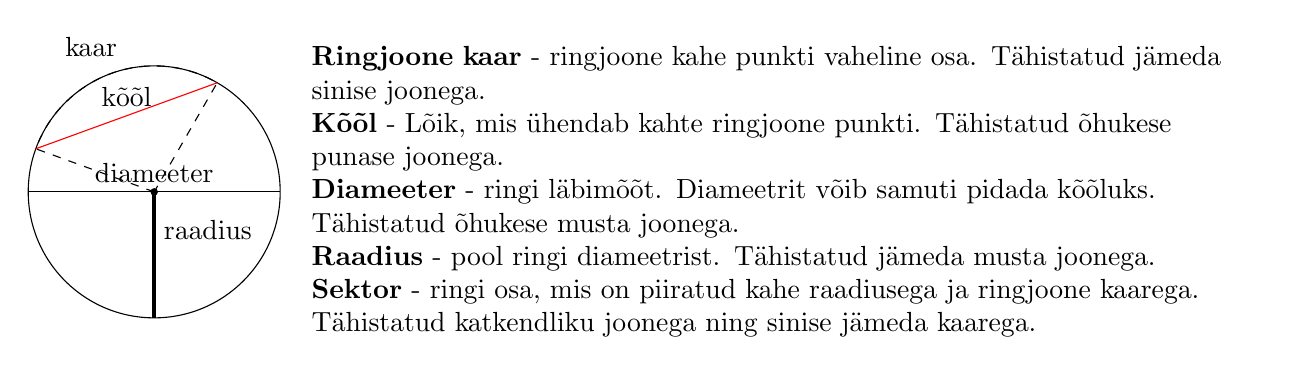
\begin{tikzpicture}[scale=0.4]
\coordinate (origin) at (0,0);
\filldraw[color= black](origin) circle(0.1);
\filldraw[color=black, fill=none](origin) circle(4);
\draw (-4,0)--(4,0);
\node[above] at (origin){diameeter};
\draw[line width=0.5mm] (0,-4)--(0,0);
\path (0,-4)--(0,0) coordinate[pos=0.7](r);
\node[right] at (r){raadius};
\centerarc[blue,line width=0.7mm](origin)(60:160:4);
\node[above] at ( -2, 4){kaar};
\draw[dashed] (origin)--(160:4) arc(160:60:4)--cycle;
\draw[thin, red] (160:4)--(60:4) node[above, black, midway]{kõõl};

\node[text width=12cm] at (20,0){ \textbf{Ringjoone kaar} - ringjoone kahe punkti vaheline osa. Tähistatud jämeda sinise joonega.\\
\textbf{Kõõl} - Lõik, mis ühendab kahte ringjoone punkti. Tähistatud õhukese punase joonega.\\
\textbf{Diameeter} - ringi läbimõõt. Diameetrit võib samuti pidada kõõluks. Tähistatud õhukese musta joonega.\\
\textbf{Raadius} - pool ringi diameetrist. Tähistatud jämeda musta joonega.\\
\textbf{Sektor} - ringi osa, mis on piiratud kahe raadiusega ja ringjoone kaarega. Tähistatud katkendliku joonega ning sinise jämeda kaarega.};
\end{tikzpicture}

\vspace{10mm}
\hspace{5mm}
\begin{tikzpicture}[scale=0.4]
\coordinate (o) at (0,0);
\draw (o) circle(4);
\filldraw[black] (o) circle(0.1);
\draw[blue, thick] (o)--(240:4) (o)--(300:4);
\draw (240:1.5) arc(240:300:1.5) node[midway,above]{$\alpha$};
\draw[red, thick] (240:4)--(90:4) (300:4)--(90:4) node[black, below=5mm]{$\beta$};
\path (240:4)--(90:4) coordinate[pos=0.7](p1);
\path (300:4)--(90:4) coordinate[pos=0.7] (p2);
\draw (p1) to [out=320, in=220] (p2) ;
\node[below] at (300:4){$B$};
\node[below] at (240:4){$A$};
\node[above] at (90:4){$C$};
\node[right] at (o){$O$};

\node[text width=12cm] at (20,0) {\textbf{Kesknurk} - nurk, mille tipp asetseb ringi keskpunktis. Joonisel on kesknurk siniste lõikude vahel tähistatud nurga $\alpha$-ga.\\
Öeldakse, et kesknurk \textbf{toetub} selle sisse jäävale kaarele. Joonisel toetub kesknurk $\alpha$ kaarele $AB$.\\
\textbf{Piirdenurk} - nurk, mis asub ringjoone ühest punktist tõmmatud kahe kõõlu vahel. Joonisel on piirdenurk punaste kõõlude vahel tähistatud nurga $\beta$-ga.\\
\vspace{2mm}
Samale kaarele tõmmatud kesknurk on \textbf{kaks korda suurem} piirdenurgast. Või teisisõnu, samale kaarele tõmmatud piirdenurk on \textbf{poole väiksem} kesknurgast.\\

\vspace{2mm}
$\boxed{\alpha=2\cdot \beta}$ või $\boxed{\beta = \dfrac{\alpha}{2}}$};
\end{tikzpicture}


\vspace{5mm}
\hspace{5mm}
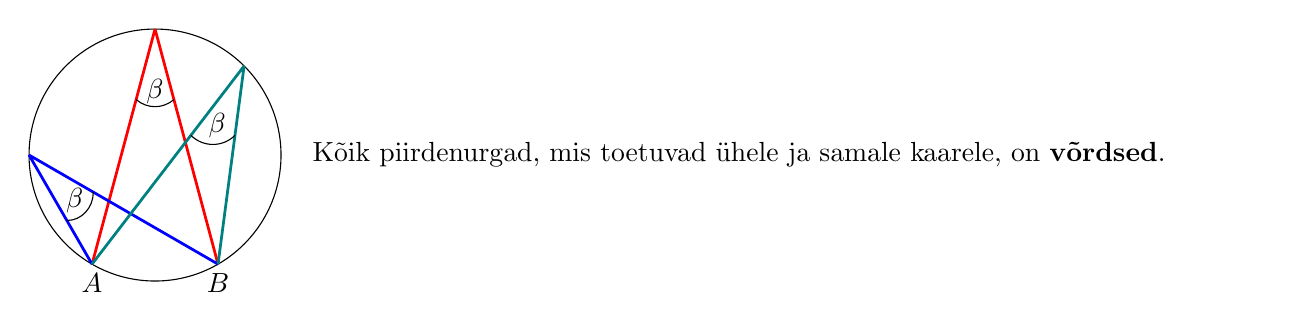
\begin{tikzpicture}[scale=0.4]
\coordinate (o) at (0,0);
\draw (o) circle(4);
\draw[red, line width=0.35mm] (240:4)--(90:4) (300:4)--(90:4) node[black, below=5mm]{$\beta$};
\path (240:4)--(90:4) coordinate[pos=0.7](p1);
\path (300:4)--(90:4) coordinate[pos=0.7] (p2);
\draw (p1) to [out=320, in=220] (p2);
\node[below] at (300:4){$B$};
\node[below] at (240:4){$A$};

\draw[blue, line width=0.35mm] (240:4)--(180:4) node[black, pos=0.58, right]{$\beta$} (300:4)--(180:4) ;
\path (240:4)--(180:4) coordinate[pos=0.4](p3);
\path (300:4)--(180:4) coordinate[pos=0.66](p4);
\draw (p3) to [out=0, in=270](p4);

\draw[teal, line width=0.35mm] (240:4)--(45:4)  (300:4)--(45:4) node[black, pos=0.7, left]{$\beta$} ;
\path (240:4)--(45:4) coordinate[pos=0.65](p5);
\path (300:4)--(45:4) coordinate[pos=0.65](p6);
\draw (p5) to [out=315, in=225](p6);

\node[text width=12cm] at(20,0) {Kõik piirdenurgad, mis toetuvad ühele ja samale kaarele, on \textbf{võrdsed}.\\
};
\end{tikzpicture}

\vspace{5mm}
\hspace{5mm}
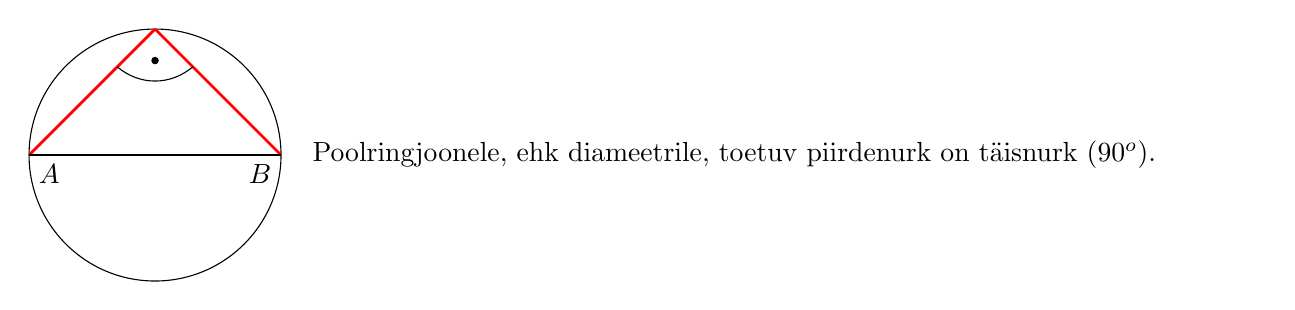
\begin{tikzpicture}[scale=0.4]
\coordinate (o) at (0,0);
\draw (o) circle(4);
\draw[red, line width=0.35mm] (180:4)--(90:4) (0:4)--(90:4);
\filldraw[black] (0,3) circle(0.1);
\path (180:4)--(90:4) coordinate[pos=0.7](p1);
\path (0:4)--(90:4) coordinate[pos=0.7] (p2);
\draw (p1) to [out=320, in=220] (p2);
\node[below right] at (180:4){$A$};
\node[below left] at (0:4){$B$};
\draw[thick] (180:4) to (0:4);
\node[text width=12cm] at (20,0) {Poolringjoonele, ehk diameetrile, toetuv piirdenurk on täisnurk ($90^{o}$).};
\end{tikzpicture}


\end{flushleft}
}}}
\end{center}


\newpage


\begin{center}
\fbox{\fbox{\parbox{6.5in}{\centering
\begin{flushleft}

\vspace{5mm}
\hspace{5mm}
\textbf{\underline{Ringjoone puutuja}}

\vspace{5mm}
\hspace{5mm}
\begin{tikzpicture}[scale=0.4, bullet/.style={circle,fill,inner sep=1pt}]

%Siit algab uus
\node[bullet,label=above right:$O$] (O) at (0,0) {};
\node (A) at (-4,5) {};
\node (B) at (0,-6){};

\draw[name path=A--B,dashed, thick] (A)--(B) node[right]{$s$};
\draw[name path=circle] (O) circle(4);

\path[name intersections = {of=circle and A--B, by={L_{1},L_{2}}}];
\node[bullet, label=below right:$L_{1}$] at (L_{1}){};
\node[bullet, label= above right:$L_{2}$] at (L_{2}){};


\draw[blue, line width=0.3mm]  (4,-4)--(4,4) node[left,blue]{$t$};
\path (4,-4)--(4,4) coordinate[pos=0.4](nurk1);
\filldraw[black] (4,0) circle(0.1) node[above left]{$P$};
\draw (0,0)--(4,0);
\node[below] at (2,0){$r$};
\path (0,0)--(4,0) coordinate[pos=0.8](nurk2);
\draw (nurk1) to [out=180, in=270](nurk2);
\filldraw[black] (3.7,-0.3) circle(0.05) node[below]{};

\node[text width=12cm] at (20,0) {\textbf{Lõikaja} - sirge, mis lõikab ringjoont kahes puntkis (joonisel katkendlik joon, sirge $s$).\\
\textbf{Puutuja} - sirge, millel on ringjoonega vaid \textbf{üks} ühine punkt (joonisel sinine sirge $t$, ning puutepunkt on $P$).\\
\vspace{2mm}
Ringjoone puutuja on alati risti ($90^{o}$ nurga all) puutepunkti tõmmatud raadiusega.};
\end{tikzpicture}

\end{flushleft}
}}}
\end{center}


\vspace{0.5cm}

\textbf{Märkmed}\\
\vspace{2mm}
\begin{mdframed}[style=graphpaper]
\vspace{13cm}
\end{mdframed}